\begin{flushleft}
Per confrontare i vari metodi abbiamo usato il seguente:
\lstinputlisting[language=Matlab]{cap_5/es6/es6.m}
\lstinputlisting[language=Matlab]{cap_5/PotenzePR.m}
Nel quale mostriamo i grafici relativi dei 3 metodi usati confrontandoli rispetto al numero di iterazioni al variare della tolleranza:
\begin{figure}[H]
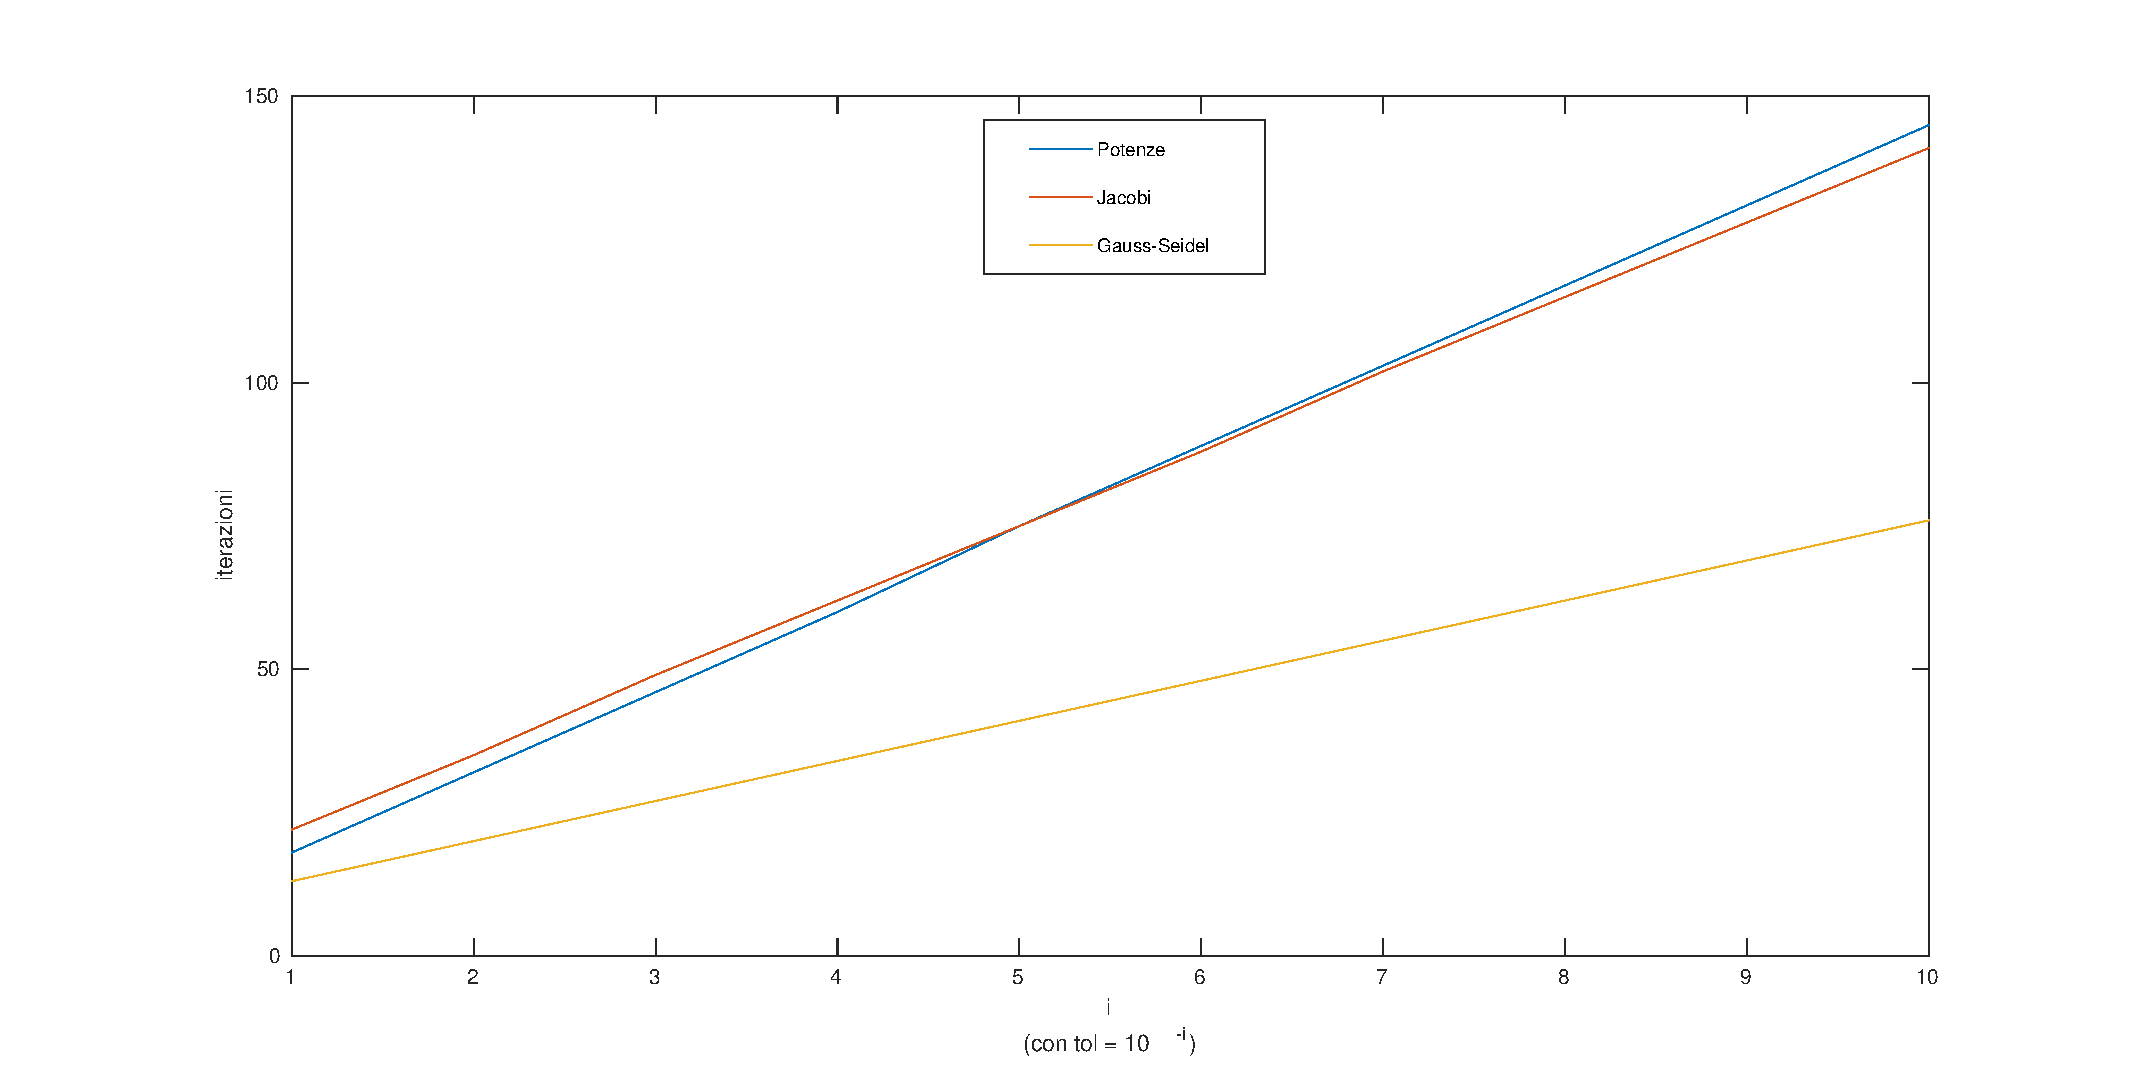
\includegraphics[width=480px, height=280px]{plot/fes56}
\end{figure}
Il metodo di Gauss-Seidell risulta il più efficiente in quanto per valori di tolleranza più piccoli converge in un numero minore delle iterazioni.
\end{flushleft}